%\vspace{4pt}
\subsection{\garand}
% overview the algorithm and introduce the main components. Each component is then described 
% in more detail in a separate paragraph. 


% reduce the white space between figure and text by 
% adjusting columnsep
% see: https://tex.stackexchange.com/questions/106144/adjusting-left-right-margins-of-a-wrapfig
\begingroup
\setlength{\columnsep}{8pt}%
	
\begin{wrapfigure}{r}{0.5\linewidth}
	\begin{center}
		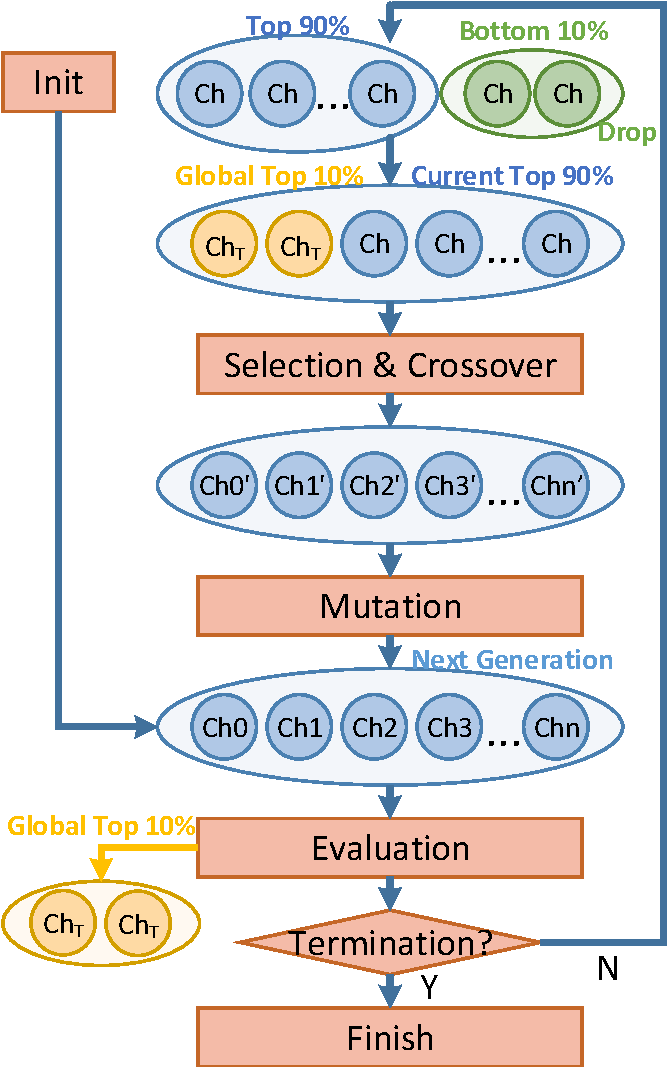
\includegraphics[width=\linewidth]{fig/pGA.pdf}
	\end{center}
	\vspace{-5pt}
	\caption{Algorithm Overview}
	\label{fig:GA}
	%\vspace{-4pt}
\end{wrapfigure}

%\begin{figure}[h]
	%\centering
	%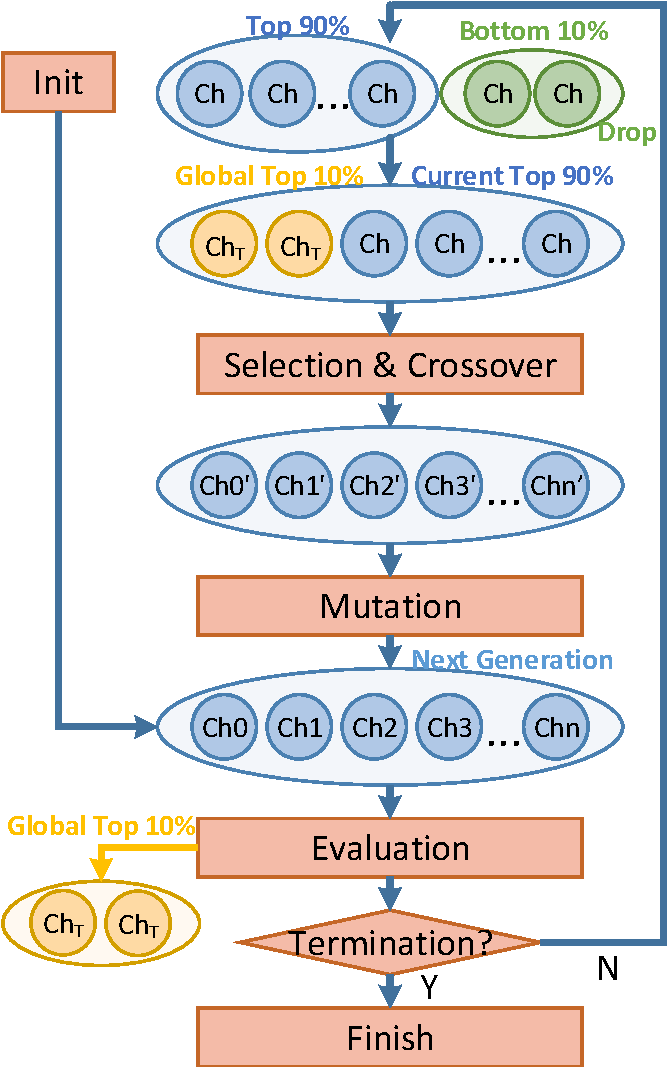
\includegraphics[width=0.75\linewidth]{fig/pGA.pdf}
	%\caption{Genetic Algorithm Overview}
	%\label{fig:GA}
%\end{figure}

\figref{fig:GA} overviews our baseline genetic algorithm. The exploration configuration is captured in a set of \emph{chromosomes}. Each chromosome captures HW/SW mapping of each function type (FT) in the domain as a set of genes. After randomly generating an initial population, the \emph{evaluation} analyzes the fitness of each chromosome using the analytical model. The evaluation tracks global top 10\% chromosomes (across all generations). They replace the bottom 10\% in a generation to start a new population. From this, \emph{Selection \& Crossover} selects pairs of promising chromosomes swaps genes among them. To further increase variation, \emph{Mutation} randomly mutates individual genes. The resulting population is evaluated again and the process repeats until the \emph{Termination} condition is reached. The next paragraphs describe the process in detail. 

\endgroup % ends the wrapfigure "reduced margin to text area"

\textbf{Chromosome Definition.} An architecture is encoded as a chromosome as a string of integers, see Eq.~\eqref{eq:ch}, representing individual genes in a fixed order. Each gene ($g_A$, $g_B$ .. $g_X$) represents whether a FT ($t_{A}$,$t_{B}$ ... $t_{X}$) is implemented in SW ($g_{I} = 0$) or in HW ($g_{I} > 0$). Adding a repeated ACC with FT existed in HW has less improvement in performance, and wastes the HW budget. To simplify the large domain design space, in this paper, each FT is at most implemented once in HW. Application to platform mapping is implicit: each actor instance of a HW-implemented FT is mapped to its HW accelerator.
As outlined in \secref{sec:Platform} "Target Platform", only HW/SW communication occurs through a common system interconnect through shared memory. Consequently, connectivity, mapping to system communication fabric or memory is not encoded as they can be inferred from the HW allocation. Connectivity within the HW partition is n:n, neither needing encoding.
%
\begin{equation}
%\vspace{-6pt}
\begin{split}
\label{eq:ch}
&Ch = \{g_A, g_B, ..., g_X \}, \left\vert{Ch}\right\vert = \left\vert{T}\right\vert \\
&g_{I} = 0, t_{I} \in SW \\
&g_{I} > 0, t_{I} \in HW \\
\end{split}
\end{equation}


\textbf{Initialization.} To form the starting population, \emph{init} randomly generates chromosomes according to the defined HW budget $N$ (i.e. $\lvert HW \rvert = N$, and $\lvert SW \rvert = \lvert T \rvert - N$). The population size is dependent on the design space, which given our assumptions is mostly impacted by the number of function types $\lvert T \rvert$. Therefore, we scale the population size dependent on domain by: $\lvert P  \rvert = \lfloor 2 * \sqrt{ \lvert T \rvert} \rfloor$.

\textbf{Evaluation / Fitness Function.} Evaluating the fitness of a single chromosome requires \emph{evaluating} each domain application on the platform encoded in the chromosome, as well as \emph{aggregating} the results. Our our analytical model \secref{sec:EvaOp} computes steady state throughput for each app. To obtain a comparable quantification across apps we consider throughput improvement: scaling throughput on the candidate platform over throughput of a pure SW platform.  The \emph{aggregation} across all applications' throughput improvement determines how well the applications are represented in the domain. As we aim for an equal representation, the applications' throughput is averaged to determine the chromosome's fitness. 

To reduce the number of generations needed for a complete exploration, \ga applies an elitist bias \cite{quan2014towards}. Chromosomes are sorted by fitness. The fittest 10\% chromosomes are promoted to a global elite pool maintained across all generations. As the global elite pool is of constant size, the most elite chromosomes displace less elites. To form a new population the bottom 10\% chromosomes are dropped and replaced with the elite pool. This allows the elite genes to breed into the next generation. 

% JH very detailed question: if one generation has a chromosome propagated to the elite pool. Then this elite chromosome will be swapped back in from the elite pool. Does the SAME chromosome then exist twice in the population (once from the top 90\% of the generation and once from the elite pool)?
% JH: yes same chromosome will exist twice -> higher chance to be chosen


\textbf{Selection \& Crossover.}
From this initial pool, a weighted roulette wheel \emph{selects} chromosomes for crossover. Fitter chromosomes (using the prior evaluation results) are more likely to be selected than less fit ones. Thus, the selection prefers fitter parents with the aim to propagate the best genes, but also allows others to foster diversity. For a selected pair of parent chromosomes, the crossover stage randomly selects which genes are inherited from each parent parents (subject to the HW budget). The selection and crossover repeats until a complete new population is formed.
% cross over is for |P| times to generate |P| new chromosomes 
% HW budget exeeded: repeat selection and cross over

\textbf{Mutation.} 
After crossover, the chromosomes are subject to mutation. It randomly selects two genes with opposite state (HW/SW allocation) and inverses their state.  

%The process of crossover and mutation repeats until a population out of only new chromosomes (result of crossover and mutation) is constructed. 
% first all cross over then all mutation 

\textbf{Termination.}
Given the new population the process repeats again with evaluating the fitness of each chromosome. The GA terminates if the best solution (i.e. the fittest chromosome from the elite pool) has not improved in the last 10 generations or the maximum number of generations (100) is reached. 
% actual implementation: OpenVX and synth are with 20 fixed generatiosn
% scaling experiments stops after 10 wihtout improvment
% observed 16 generations for small, 29 for large (100 types)
% max number is theoretical (not actually implemented)


%GS disabled the stuff below as it basically repeats as intro in the next section

%While a random genetic algorithm can perform well for an application DSE, we have found that it still takes too long for domain-DSE as it relies on random mutation without guidance. To improve exploration speed, we introduce a guided local search for the mutation. The next three sections discuss alternative approaches for the guided local search. 

%Heuristic Guided Mutation
